\documentclass[12pt,letterpaper]{article}

\usepackage[utf8]{inputenc}
\usepackage[T1]{fontenc}
\usepackage[spanish,es-nodecimaldot]{babel}
\usepackage{geometry}
\usepackage{graphicx}
\usepackage{booktabs}
\usepackage{array}
\usepackage{xcolor}
\usepackage{hyperref}
\usepackage{enumitem}
\usepackage{float}
\usepackage{longtable}
\usepackage{listings}
\usepackage{caption}

\geometry{margin=2.4cm}
\graphicspath{{diagrams/}{docs/diagrams/}{./}{docs/}}
\hypersetup{
  colorlinks=false,
  pdfborder={0 0 0}
}
\definecolor{blacktext}{HTML}{000000}
\definecolor{lightgray}{HTML}{F2F2F2}
\definecolor{midgray}{HTML}{666666}
\pagecolor{white}
\color{blacktext}

\lstdefinestyle{bwcode}{
  basicstyle=\ttfamily\small,
  backgroundcolor=\color{lightgray},
  frame=single,
  rulecolor=\color{black},
  breaklines=true,
  columns=fullflexible,
  keepspaces=true,
  showstringspaces=false
}
\lstset{style=bwcode}
\setlist[itemize]{leftmargin=*, itemsep=2pt, topsep=4pt}
\setlist[enumerate]{leftmargin=*, itemsep=2pt, topsep=4pt}
\captionsetup{labelfont=bf, textfont=it}

\begin{document}

\begin{titlepage}
\pagenumbering{gobble}
\thispagestyle{empty}
\centering
\vspace*{1.2cm}

\begin{minipage}{0.18\textwidth}
\centering

\includegraphics[width=\linewidth,height=2.9cm,keepaspectratio]{escudo_IPN.png}
\end{minipage}
\hfill
\begin{minipage}{0.58\textwidth}
\centering
{\Large\textbf{INSTITUTO POLITÉCNICO NACIONAL}}\\[0.35cm]
{\large\textbf{ESCUELA SUPERIOR DE CÓMPUTO}}
\end{minipage}
\hfill
\begin{minipage}{0.18\textwidth}
\centering

\includegraphics[width=\linewidth,height=2.2cm,keepaspectratio]{logoESCOM2x.png}
\end{minipage}

\vspace{3.0cm}
\rule{0.88\textwidth}{0.4pt}

\vspace{0.65cm}
{\Huge\textbf{Proyecto Final}}

\vspace{0.65cm}
\rule{0.88\textwidth}{0.4pt}

\vspace{1.8cm}
{\large\textbf{Unidad de Aprendizaje:} \textit{Internet de las cosas/Embedded Systems}}

\vspace{1.2cm}
{\large\textbf{Profesora:} \textit{Miguel Ángel Alemán Arce}}

\vspace{1.4cm}
{\large\textbf{Integrantes:}}

\vspace{0.8cm}
{\large\textit{Daniel Soria González}}

\vfill
{\large\textbf{Grupo:} \textit{6CM3}}

\vspace{0.8cm}
{\normalsize \today}
\end{titlepage}
\pagenumbering{arabic}

\tableofcontents
\newpage

\section{Resumen}

Este proyecto implementa un sistema IoT para monitorear la apertura y cierre de siete compartimentos mediante sensores magnéticos tipo \textit{reed switch}. La arquitectura se diseñó con tres roles MQTT bien separados: un nodo publicador en ESP32, un broker Mosquitto y un nodo suscriptor con interfaz web. El ESP32 lee el estado físico de cada compartimento, publica eventos individuales y un resumen global; el dashboard recibe esos mensajes, muestra el estado en tiempo real y activa una alarma digital cuando detecta al menos un compartimento abierto.

La solución cubre los requisitos principales de la asignación: uso de hardware embebido, comunicación mediante MQTT, definición jerárquica de tópicos, selección justificada de QoS, reacción de un subscriber ante los datos recibidos y evidencias de despliegue. Además, incluye elementos opcionales de valor agregado: contenedores Docker para Mosquitto y el dashboard, una interfaz web propia, eventos en tiempo real y comandos remotos para solicitar sincronización o habilitar/deshabilitar el monitoreo.

\section{Introducción y contexto}

En un sistema de Internet de las Cosas, los nodos suelen tener responsabilidades pequeñas y comunicarse a través de una red. MQTT es adecuado para este tipo de proyectos porque usa un modelo de publicación/suscripción: el dispositivo que mide no necesita conocer directamente a la aplicación que visualiza, y la aplicación que reacciona no necesita conectarse al sensor de forma directa. Ambos se comunican mediante un broker que recibe, filtra y distribuye mensajes por tópicos.

El caso desarrollado consiste en supervisar siete compartimentos. Cada compartimento tiene un sensor reed switch que cambia su lectura cuando el imán asociado se separa o se acerca. En términos simples, el sensor permite saber si una puerta, tapa o cajón está abierto o cerrado. El ESP32 convierte esas lecturas eléctricas en mensajes JSON publicados por MQTT. Después, el dashboard interpreta esos mensajes para presentar una vista clara al operador y generar una alarma cuando el estado del sistema lo requiere.

\section{Objetivos}

\subsection{Objetivo general}

Diseñar e implementar una arquitectura IoT basada en MQTT para monitorear siete compartimentos físicos y reaccionar en tiempo real mediante una alarma digital y una interfaz de control.

\subsection{Objetivos específicos}

\begin{itemize}
  \item Implementar el rol de \textit{publisher} en un ESP32 programado en C++ con el framework Arduino.
  \item Configurar Eclipse Mosquitto como broker MQTT local o contenedorizado.
  \item Implementar un \textit{subscriber} en Python que actualice un dashboard web y publique el estado de una alarma digital.
  \item Definir un árbol de tópicos jerárquico, entendible y alineado con el dominio del proyecto.
  \item Aplicar QoS 1 en mensajes donde la pérdida de información puede afectar la consistencia del estado mostrado.
  \item Documentar la arquitectura, la topología de red, el flujo de operación, las pruebas esperadas y las conclusiones.
\end{itemize}

\section{Descripción general del sistema}

El sistema se divide en tres capas. La primera es la capa de hardware, formada por el ESP32, los siete reed switches y un LED indicador. La segunda es la capa de red y mensajería, donde Mosquitto recibe y distribuye los mensajes MQTT. La tercera es la capa de aplicación, formada por el dashboard web y la lógica de alarma.

El ESP32 no envía datos continuamente sin sentido; revisa las entradas digitales y solo publica cambios cuando detecta una transición estable después de un tiempo de antirrebote de 60 ms. Esto evita que una vibración o un falso contacto se convierta en varios eventos. También publica un \textit{heartbeat} cada 5 segundos para informar que el dispositivo sigue vivo, junto con datos útiles como RSSI, tiempo encendido y cantidad de compartimentos abiertos.

\begin{figure}[H]
  \centering
  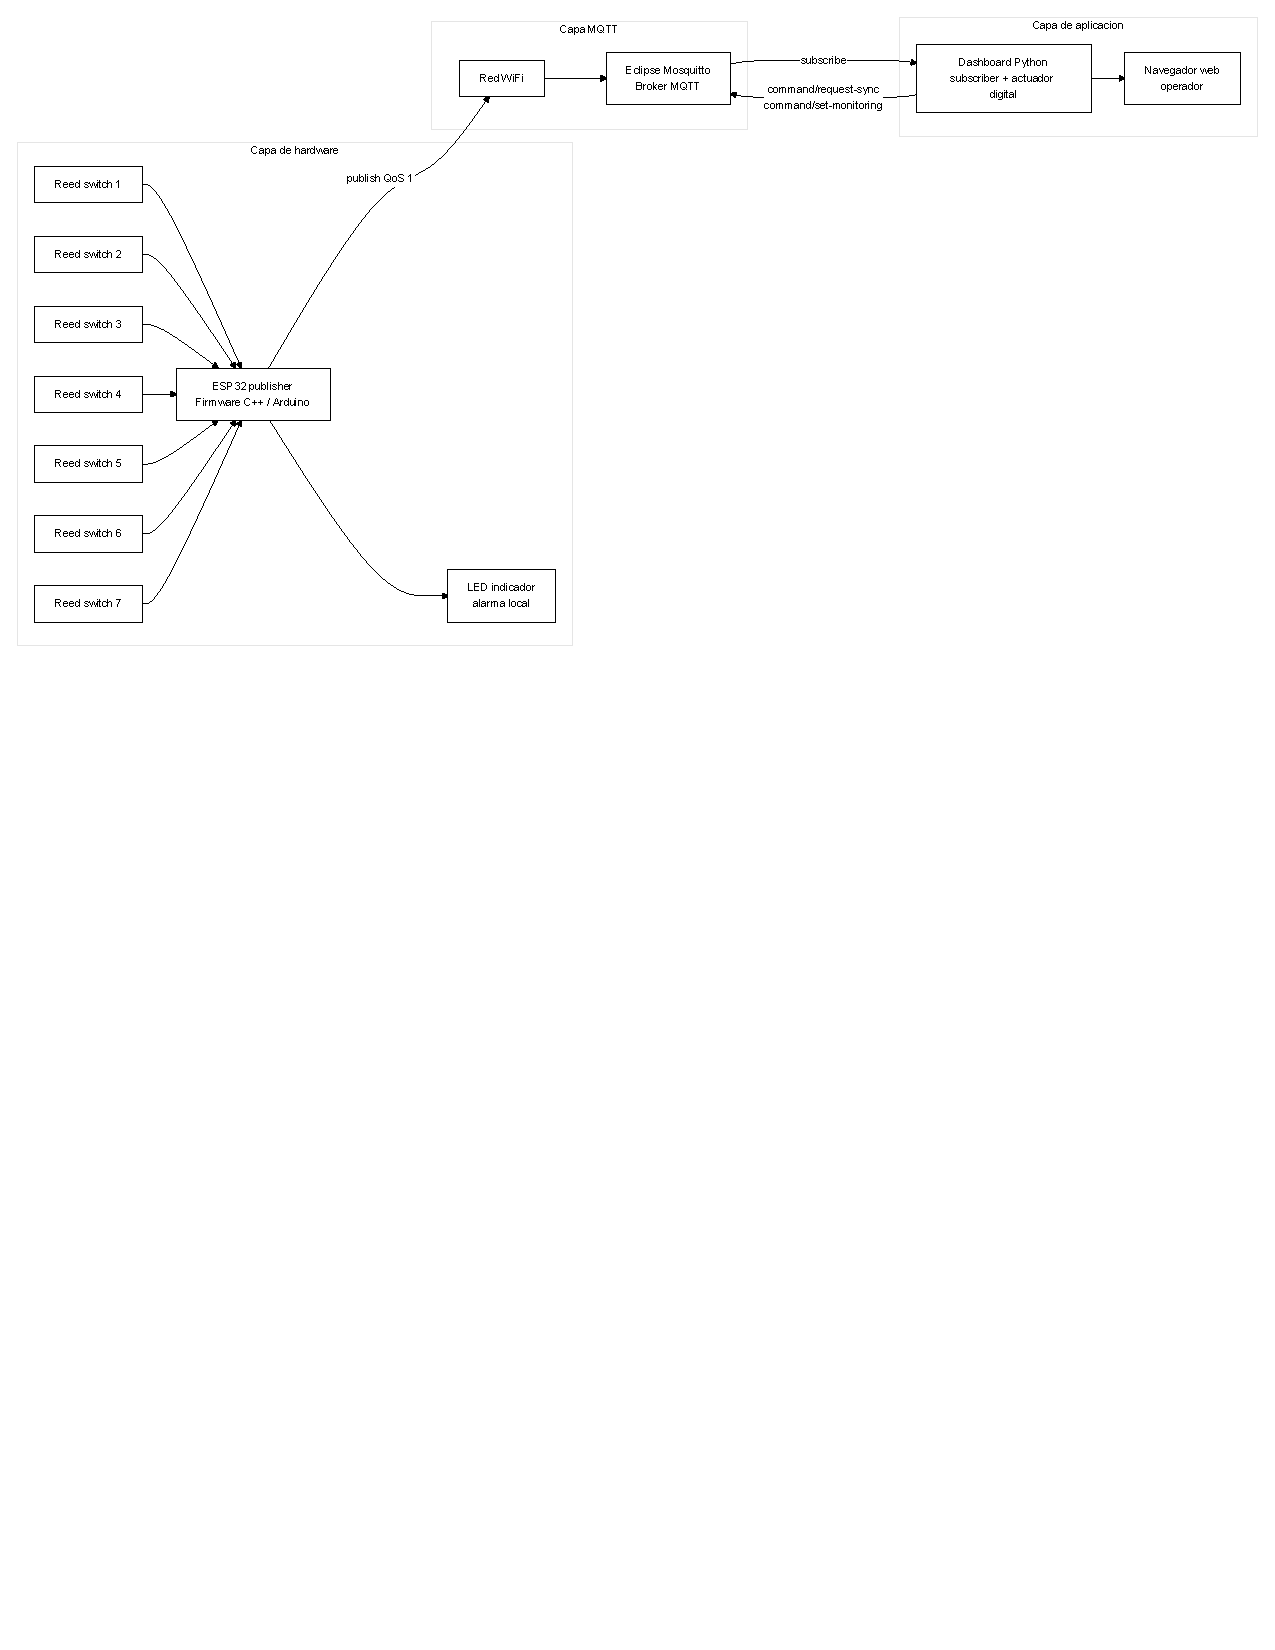
\includegraphics[width=0.96\textwidth]{arquitectura.pdf}
  \caption{Arquitectura general del sistema IoT.}
  \label{fig:arquitectura}
\end{figure}

\section{Capa de hardware e infraestructura}

\subsection{Nodo publicador ESP32}

El publicador se implementó en un ESP32 usando C++ y el framework Arduino. Su función es leer siete entradas digitales conectadas a reed switches. En este proyecto, una lectura alta se interpreta como compartimento abierto. Para los compartimentos 3 al 7 se usa \texttt{INPUT\_PULLUP}; para los GPIO 34 y 35 se requiere resistencia externa de pull-up, porque esos pines del ESP32 son solo de entrada y no tienen pull-up interno.

\begin{table}[H]
\centering
\caption{Asignación de sensores a pines GPIO.}
\begin{tabular}{ccc}
\toprule
\textbf{Compartimento} & \textbf{GPIO} & \textbf{Observación eléctrica} \\
\midrule
1 & 34 & Requiere pull-up externo \\
2 & 35 & Requiere pull-up externo \\
3 & 32 & Usa pull-up interno \\
4 & 33 & Usa pull-up interno \\
5 & 25 & Usa pull-up interno \\
6 & 26 & Usa pull-up interno \\
7 & 27 & Usa pull-up interno \\
\bottomrule
\end{tabular}
\end{table}

El firmware mantiene una estructura de estado por sensor con tres datos importantes: el estado abierto/cerrado estable, la última lectura instantánea y el tiempo en que ocurrió el último rebote. Esta decisión hace que el ESP32 no dependa de retardos bloqueantes, por lo que puede seguir atendiendo MQTT y WiFi mientras procesa los sensores.

\subsection{Broker Mosquitto}

El broker MQTT se configuró con Eclipse Mosquitto. La configuración habilita el puerto 1883 para MQTT estándar y el puerto 9001 para WebSocket. También se activa persistencia, lo cual permite conservar datos retenidos y estado básico del broker entre reinicios del contenedor. Para el entorno de laboratorio se permite conexión anónima, lo que simplifica la demostración; en un despliegue real se recomendaría activar usuarios, contraseñas y, si aplica, TLS.

\subsection{Subscriber y actuador digital}

El subscriber se implementó en Python con la biblioteca \texttt{paho-mqtt}. La aplicación se conecta al broker, se suscribe a los tópicos del publisher y mantiene un estado interno del sistema. Cuando un compartimento pasa a abierto y el monitoreo está habilitado, la aplicación activa una alarma digital. Esa alarma se publica en MQTT bajo el tópico \texttt{actuator/alarm} y también se refleja en el dashboard web.

El dashboard ofrece tres acciones principales para el operador: reconocer la alarma, solicitar una sincronización completa del estado y activar o desactivar el monitoreo. Estas acciones no modifican directamente el firmware por cable o por una API privada; se envían como comandos MQTT, respetando el mismo modelo desacoplado de la arquitectura.

\section{Topología de red}

La topología se basa en una red local WiFi. El ESP32 se conecta como estación a la red del laboratorio, el broker se ejecuta en una computadora o SBC dentro de la misma red y el dashboard puede ejecutarse en el mismo host o en un contenedor separado. El operador accede al dashboard mediante HTTP en el puerto 8080.

\begin{figure}[H]
  \centering
  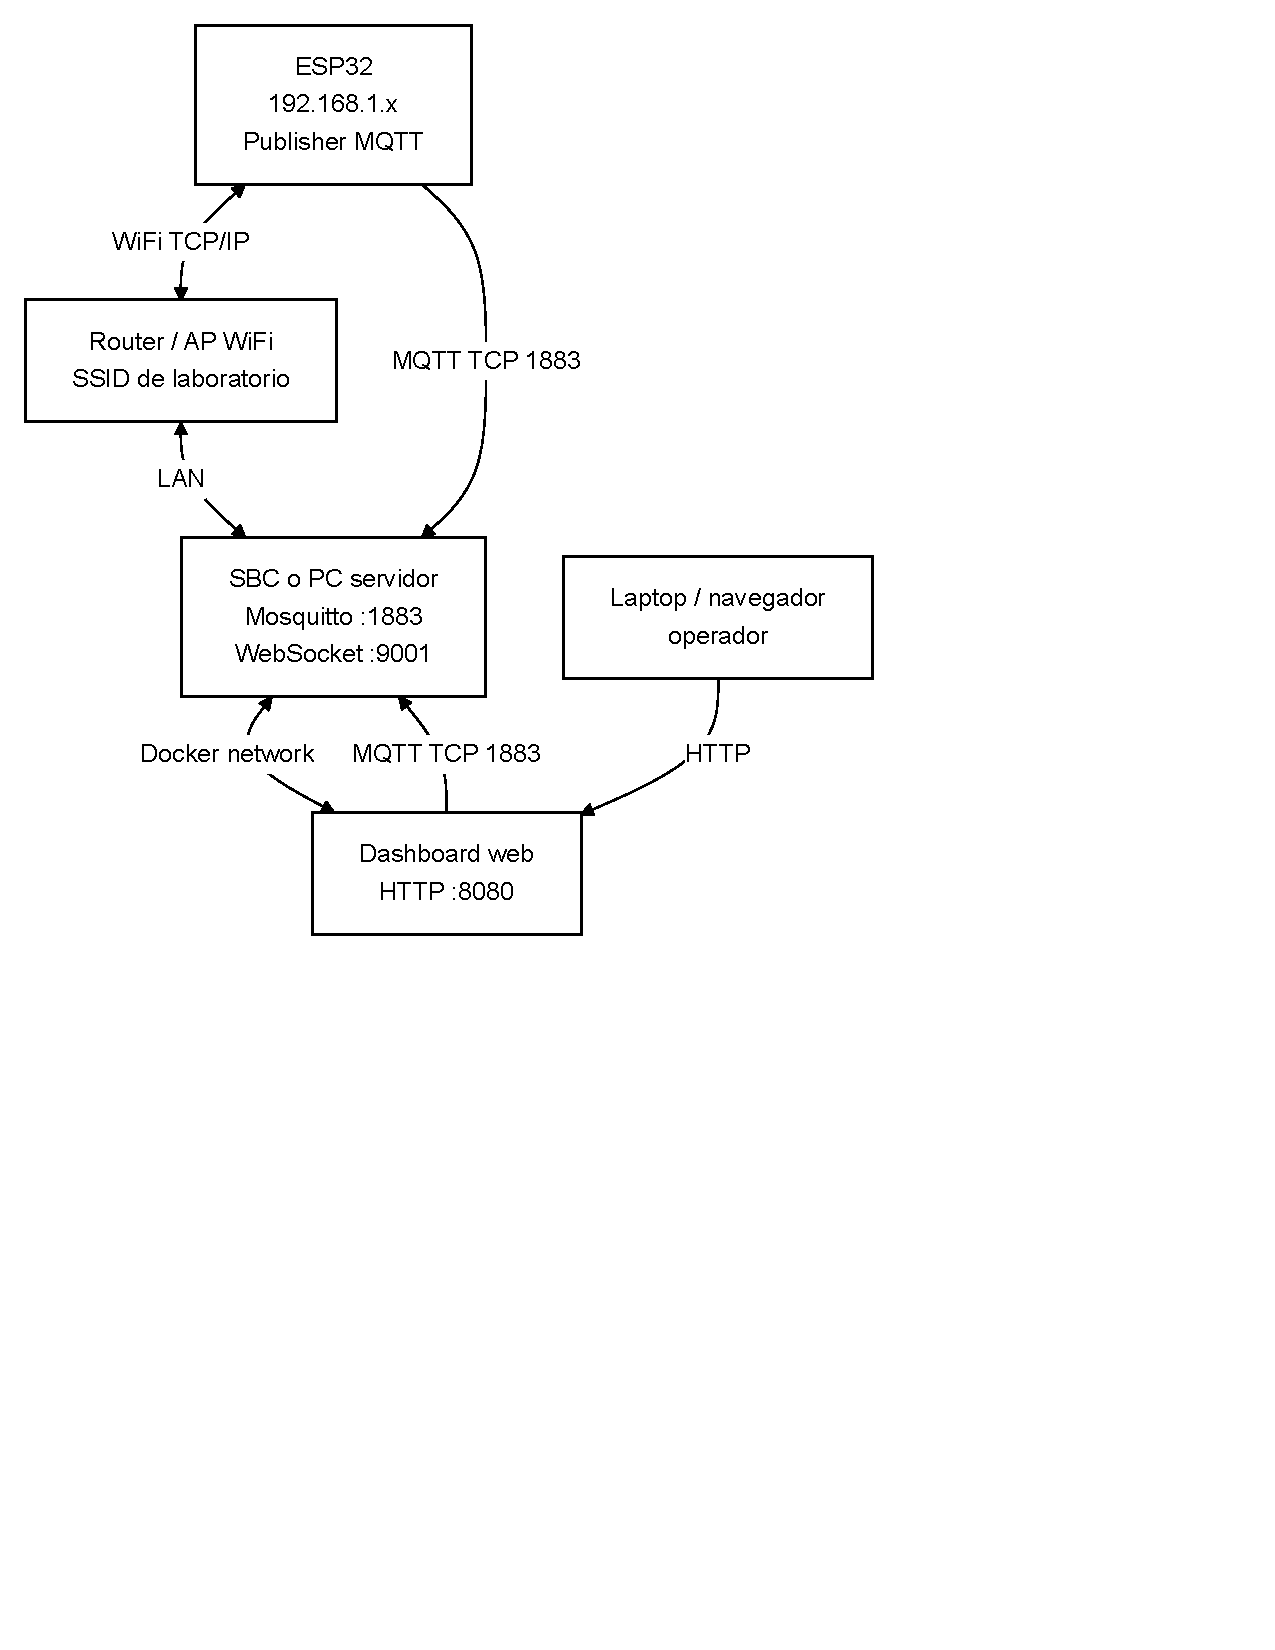
\includegraphics[width=0.90\textwidth]{topologia.pdf}
  \caption{Topología de red propuesta para laboratorio.}
  \label{fig:topologia}
\end{figure}

La comunicación crítica entre ESP32 y broker ocurre sobre TCP en el puerto 1883. El firmware incluso prueba la conexión TCP antes de intentar la conexión MQTT, lo que ayuda a distinguir entre una falla de red y una falla propia del protocolo MQTT. Esta verificación es útil en laboratorio porque permite diagnosticar problemas típicos como IP incorrecta, broker apagado o dispositivos conectados a redes distintas.

\section{Árbol de tópicos MQTT}

El árbol de tópicos se diseñó con una raíz común: \texttt{escom/iot/equipo7/reed-monitor}. Esta raíz identifica la institución, el dominio IoT, el equipo y el tipo de sistema. Debajo de esa raíz se separan los tópicos por responsabilidad: estado del publisher, sensores, comandos, actuador y estado del subscriber.

\begin{figure}[H]
  \centering
  
\includegraphics[width=0.92\textwidth]{topicos.pdf}
  \caption{Árbol jerárquico de tópicos MQTT.}
  \label{fig:topicos}
\end{figure}

\begin{longtable}{p{0.36\textwidth}p{0.18\textwidth}p{0.36\textwidth}}
\caption{Descripción funcional de tópicos principales.}\\
\toprule
\textbf{Tópico} & \textbf{Dirección} & \textbf{Uso} \\
\midrule
\endfirsthead
\toprule
\textbf{Tópico} & \textbf{Dirección} & \textbf{Uso} \\
\midrule
\endhead
\texttt{publisher/status} & ESP32 a broker & Indica si el publicador está en línea e informa su IP. \\
\texttt{sensor/compartment/N} & ESP32 a broker & Publica el estado individual del compartimento N. \\
\texttt{sensor/summary} & ESP32 a broker & Envía una fotografía completa de los siete compartimentos. \\
\texttt{sensor/heartbeat} & ESP32 a broker & Reporta vida del nodo, RSSI, uptime y cantidad de abiertos. \\
\texttt{command/request-sync} & Dashboard a ESP32 & Solicita republicar todos los estados y resumen. \\
\texttt{command/set-monitoring} & Dashboard a ESP32 & Habilita o inhibe el monitoreo remoto. \\
\texttt{actuator/alarm} & Dashboard a broker & Publica el estado actual de la alarma digital. \\
\texttt{subscriber/status} & Dashboard a broker & Indica si el dashboard está en línea. \\
\bottomrule
\end{longtable}

\section{Selección de QoS y mensajes retenidos}

El proyecto usa QoS 1 en las suscripciones y publicaciones importantes. QoS 1 significa que el broker debe recibir el mensaje al menos una vez. Es una decisión equilibrada: mejora la confiabilidad frente a QoS 0, pero evita la complejidad y sobrecarga de QoS 2. En este sistema, recibir un duplicado ocasional es aceptable porque los mensajes contienen estado y secuencia; perder un evento de apertura sería más problemático.

Los mensajes de disponibilidad y algunos estados se publican como retenidos. Esto permite que un subscriber que se conecte después reciba inmediatamente el último estado conocido sin esperar a que ocurra otro cambio físico. Para un dashboard, esta característica es importante porque evita iniciar con una pantalla vacía o inconsistente.

\begin{table}[H]
\centering
\caption{Criterio de QoS y retención.}
\begin{tabular}{p{0.34\textwidth}cp{0.38\textwidth}}
\toprule
\textbf{Mensaje} & \textbf{QoS} & \textbf{Justificación} \\
\midrule
Estado de publisher y subscriber & 1 & La disponibilidad debe conocerse aunque el cliente se conecte después. \\
Estado individual de compartimento & 1 & Un cambio físico no debe perderse durante la demostración. \\
Resumen de sensores & 1 & Recupera consistencia si algún evento individual no se procesó. \\
Comandos de sincronización y monitoreo & 1 & El comando debe llegar al nodo correspondiente al menos una vez. \\
Heartbeat & 1 o entrega normal & Sirve para diagnóstico periódico; su valor envejece rápido. \\
\bottomrule
\end{tabular}
\end{table}

\section{Flujo de operación}

El flujo inicia cuando un reed switch cambia de estado. El ESP32 detecta la lectura, espera el periodo de debounce y compara contra el último estado estable. Si realmente hubo cambio, incrementa un número de secuencia, publica el evento individual y publica un resumen general. El broker no interpreta el contenido; solo enruta los mensajes a los clientes suscritos.

El dashboard recibe el mensaje, actualiza su estado interno y recalcula la alarma. Si existe al menos un compartimento abierto y el monitoreo está habilitado, la alarma queda activa. El operador puede reconocer la alarma desde la interfaz, pero ese reconocimiento no cierra el compartimento; solamente registra que la alerta fue vista. La alarma se limpia cuando ya no hay compartimentos abiertos o cuando el monitoreo se desactiva.

\begin{figure}[H]
  \centering
  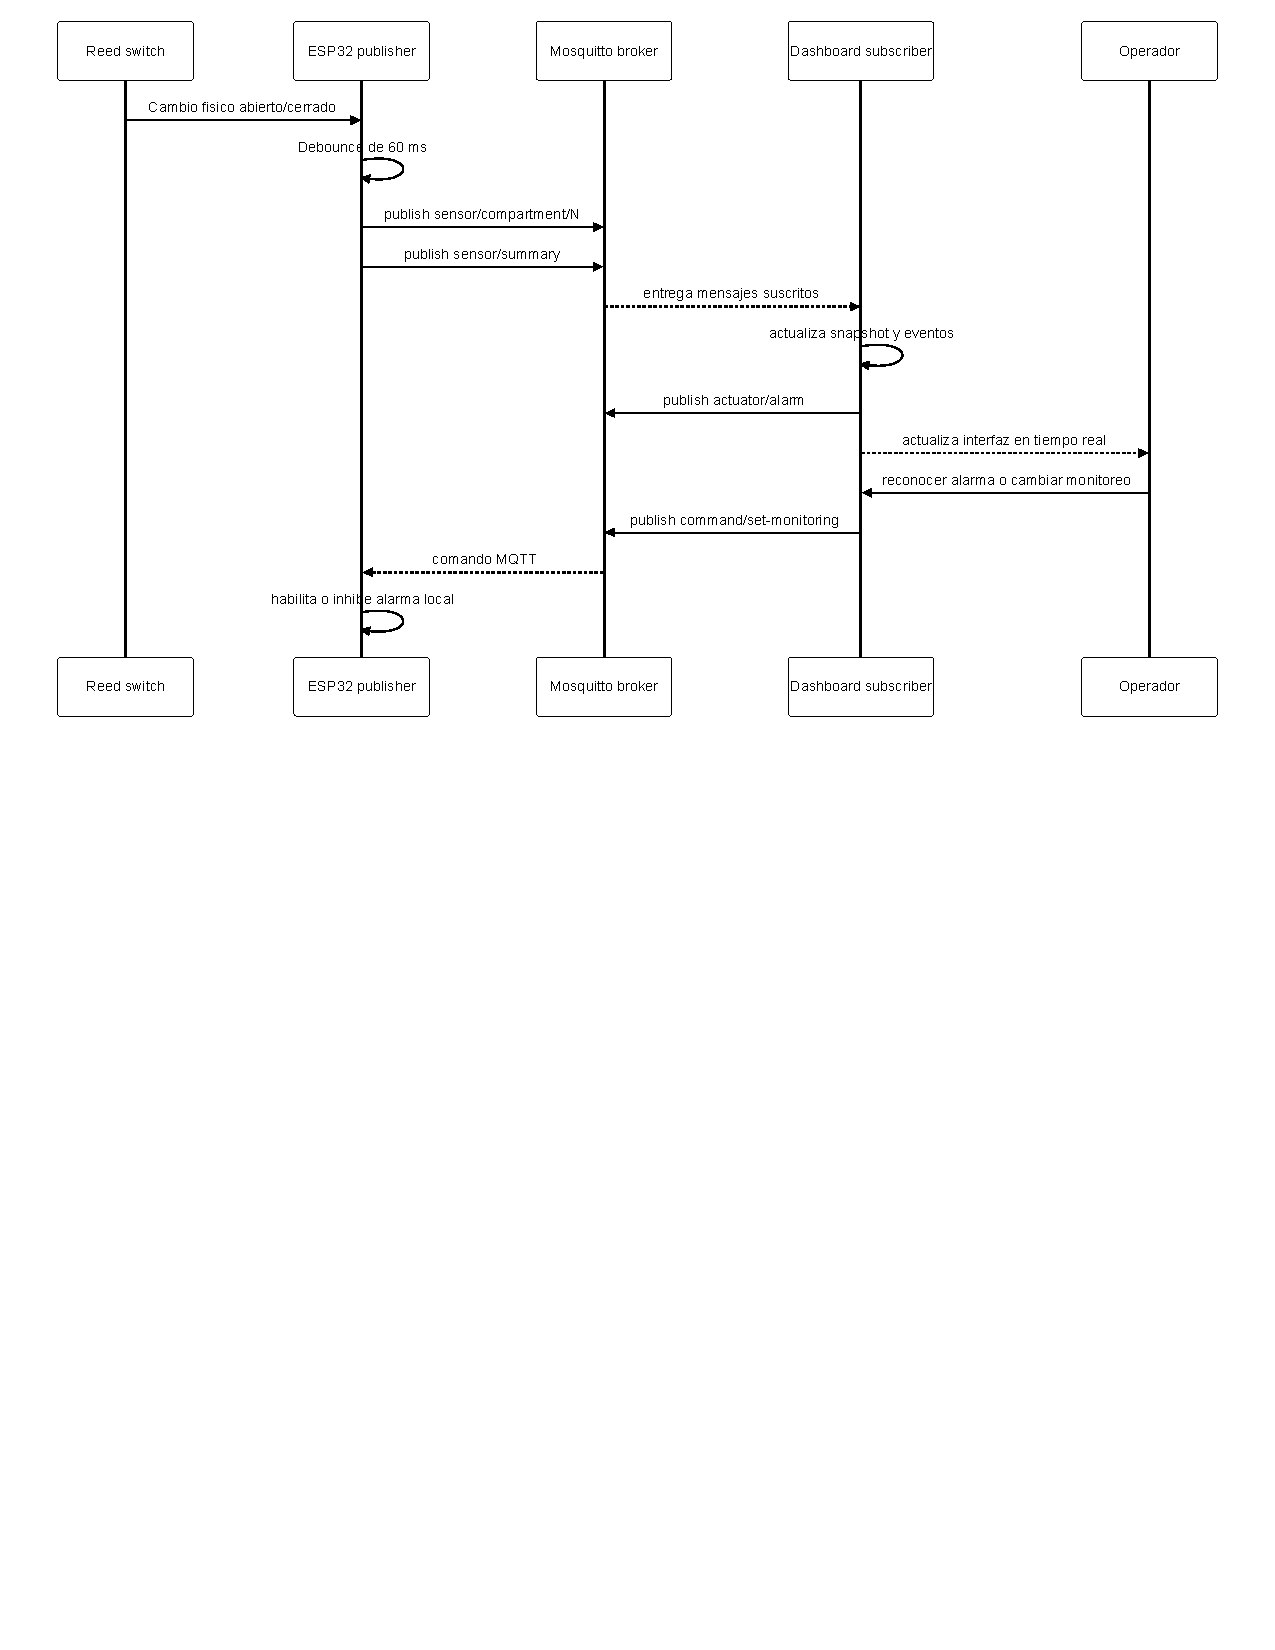
\includegraphics[width=0.96\textwidth]{flujo.pdf}
  \caption{Secuencia principal de operación y control.}
  \label{fig:flujo}
\end{figure}

\section{Despliegue y ejecución}

El proyecto puede ejecutarse con Docker Compose. El archivo de composición levanta dos servicios: \texttt{mosquitto} y \texttt{dashboard}. Mosquitto expone los puertos 1883 y 9001; el dashboard expone el puerto 8080. Esta forma de despliegue reduce errores de instalación porque el broker y la aplicación se levantan con una configuración repetible.

\begin{lstlisting}[language=bash,caption={Ejecución con Docker Compose.}]
docker compose up --build
\end{lstlisting}

Para una ejecución local del subscriber sin Docker, se crea un entorno de Python, se instalan dependencias y se ejecuta el módulo de la aplicación:

\begin{lstlisting}[language=bash,caption={Ejecución local del dashboard.}]
python -m venv .venv
.venv\Scripts\activate
pip install -r subscriber/requirements.txt
python -m subscriber.app
\end{lstlisting}

El firmware del ESP32 debe cargarse desde Arduino IDE o PlatformIO, ajustando previamente la red WiFi y la dirección IP del broker. En el estado actual del código, el broker está configurado en \texttt{192.168.1.85} y el puerto MQTT en \texttt{1883}. Si el broker cambia de equipo o red, esa IP debe actualizarse antes de flashear.

\section{Análisis de resultados y pruebas de conectividad}

Las pruebas de conectividad deben demostrar que cada capa cumple su función. Primero se valida red básica con \texttt{ping} al host del broker. Después se verifica que Mosquitto acepte conexiones en el puerto 1883. Luego se observa el tráfico MQTT con un cliente de consola, y finalmente se comprueba que el dashboard reaccione al abrir y cerrar compartimentos.

\begin{lstlisting}[language=bash,caption={Comandos sugeridos para validar MQTT.}]
ping <ip-del-broker>
mosquitto_sub -h <ip-del-broker> -t "escom/iot/equipo7/reed-monitor/#" -v
\end{lstlisting}

\begin{table}[H]
\centering
\caption{Matriz de validación para laboratorio.}
\begin{tabular}{p{0.26\textwidth}p{0.34\textwidth}p{0.26\textwidth}}
\toprule
\textbf{Prueba} & \textbf{Resultado esperado} & \textbf{Evidencia} \\
\midrule
Ping al broker & Respuesta estable desde el equipo de pruebas. & Latencia y paquetes recibidos. \\
Conexión MQTT del ESP32 & Mensaje \texttt{publisher/status} en línea. & Consola serial y \texttt{mosquitto\_sub}. \\
Apertura de compartimento & Evento en \texttt{sensor/compartment/N}. & Dashboard marca compartimento abierto. \\
Cierre de compartimento & Evento de cierre y reducción de \texttt{open\_count}. & Dashboard vuelve a estado normal. \\
Solicitud de sincronización & Republicación de estados y resumen. & Mensaje en \texttt{sensor/summary}. \\
Desactivar monitoreo & La alarma queda inhibida aunque haya apertura. & Estado de monitoreo en falso. \\
\bottomrule
\end{tabular}
\end{table}

Desde el punto de vista funcional, el uso combinado de eventos individuales y resumen global mejora la robustez. El evento individual permite reaccionar rápido a un cambio específico, mientras que el resumen permite reconstruir el estado completo del sistema. El heartbeat agrega una señal de diagnóstico: si deja de recibirse, el dashboard o el operador pueden sospechar pérdida de WiFi, apagado del ESP32 o falla del broker.

\section{Consideraciones de seguridad y mejora}

Para laboratorio se permite \texttt{allow\_anonymous true} en Mosquitto, lo cual simplifica la práctica. Sin embargo, en un entorno real esto debe cambiarse. Un broker sin autenticación permite que cualquier cliente en la misma red publique comandos, desactive monitoreo o genere falsas alarmas. La mejora natural sería crear usuarios MQTT, usar contraseñas y separar permisos de publicación y suscripción por tópico.

Otra mejora posible es almacenar histórico de eventos en una base de datos ligera. El dashboard ya conserva eventos recientes en memoria, pero esos datos se pierden al reiniciar la aplicación. Para analítica real se podría integrar SQLite, InfluxDB o un servicio similar. También se puede ampliar el dashboard con gráficas de aperturas por compartimento, tiempos promedio de apertura y alertas por desconexión prolongada.

\section{Conclusiones}

El proyecto cumple con la arquitectura solicitada para un sistema IoT basado en MQTT. El ESP32 funciona como nodo publicador embebido, Mosquitto cumple el rol de broker y el dashboard Python actúa como subscriber y actuador digital. La separación de responsabilidades facilita depurar el sistema, cambiar el dashboard sin reprogramar el sensor y observar el tráfico MQTT con herramientas estándar.

La selección de QoS 1 es adecuada para el dominio del problema porque los eventos de apertura y cierre son relevantes para el estado de seguridad del sistema. La publicación de resúmenes y mensajes retenidos ayuda a mantener consistencia cuando un cliente se conecta tarde o necesita resincronizarse. Además, Docker Compose aporta portabilidad y el dashboard propio cubre el componente opcional de visualización y control.

Como trabajo futuro, se recomienda reforzar seguridad MQTT, registrar histórico persistente, medir latencia real entre apertura física y actualización del dashboard, y documentar con capturas o video la demostración final en laboratorio. Con esas evidencias, el reporte quedaría alineado con la rúbrica de funcionalidad, arquitectura, documentación y defensa práctica.

\end{document}
